\documentclass[preview]{standalone}
\usepackage{tikz,fullpage,tikz-network,verbatim}
\usetikzlibrary{arrows, petri, topaths, calc, angles, quotes}
\begin{document}
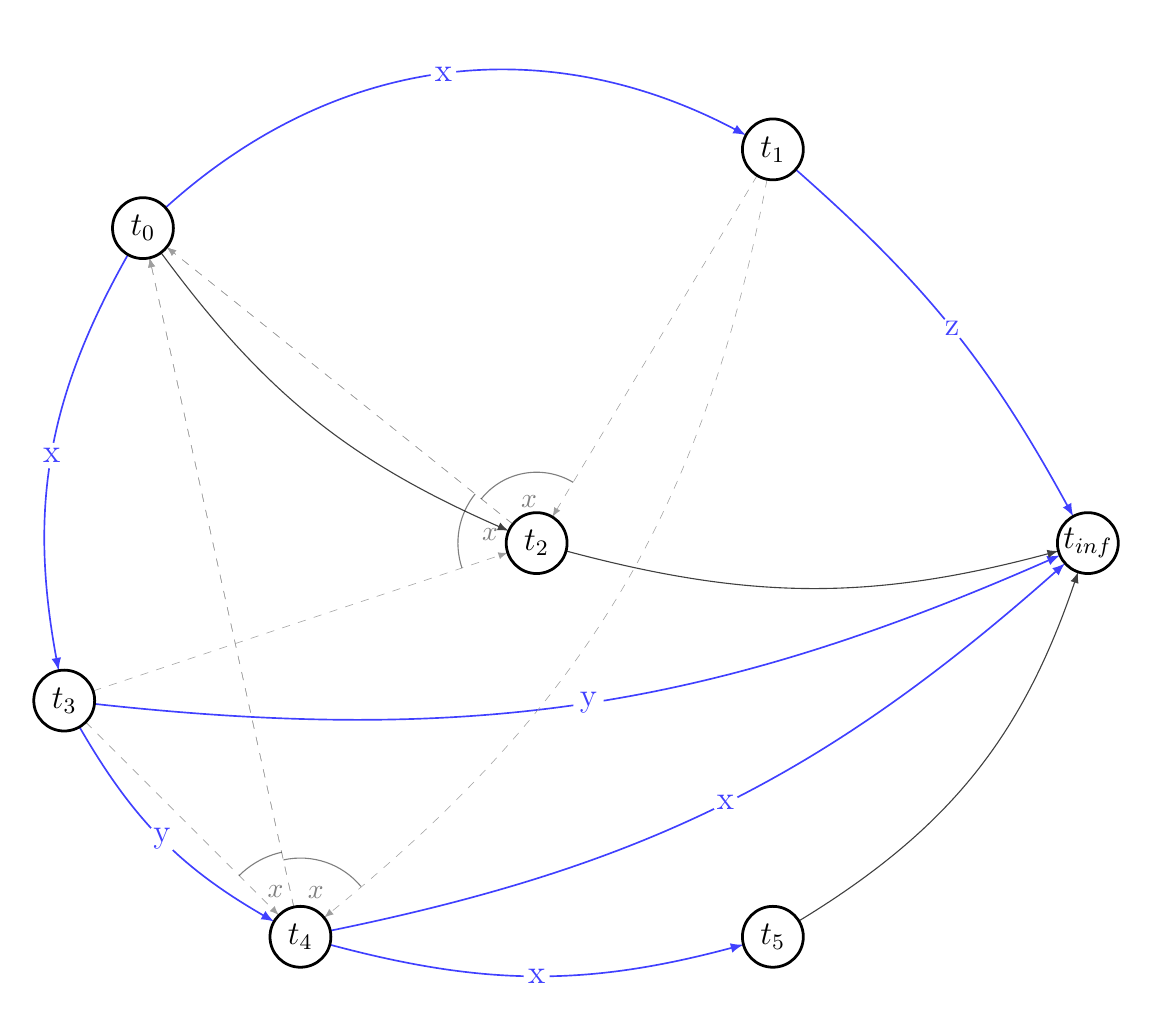
\begin{tikzpicture}[scale=1,transform shape]
  %\draw (0, 0) grid (15, 10);

  \SetVertexStyle[FillColor=white,TextFont=\large,MinSize=22]
  \Vertex[x=3 ,y=9, label=$t_0$]{t0}
  \Vertex[x=11,y=10,label=$t_1$]{t1}
  \Vertex[x=8 ,y=5, label=$t_2$]{t2}
  \Vertex[x=2 ,y=3, label=$t_3$]{t3}
  \Vertex[x=5 ,y=0, label=$t_4$]{t4}
  \Vertex[x=11,y=0, label=$t_5$]{t5}
  \Vertex[x=15,y=5, label=$t_{inf}$]{tinf}

  \SetEdgeStyle[TextFont=\large,LineWidth=0.6pt,InnerSep=0.5pt,Color=blue!75]
  \Edge[label=x,Direct,bend=35](t0)(t1)
  \Edge[label=x,Direct,bend=-20](t0)(t3)
  \Edge[label=y,Direct,bend=-15](t3)(t4)
  \Edge[label=x,Direct,bend=-15](t4)(t5)
  \Edge[label=z,Direct,bend=10](t1)(tinf)
  \Edge[label=y,Direct,bend=-15](t3)(tinf)
  \Edge[label=x,Direct,bend=-15](t4)(tinf)

  \SetEdgeStyle[TextFont=\large,LineWidth=0.4pt,InnerSep=0.5pt,Color=black!75]
  \Edge[Direct,bend=-15](t0)(t2)
  \Edge[Direct,bend=-15](t2)(tinf)
  \Edge[Direct,bend=-20](t5)(tinf)

  % Choices:
  \SetEdgeStyle[TextFont=\large,LineWidth=0.2pt,InnerSep=0.5pt,Color=gray!75]

  % t1 -> t2 -> t0 [label=x]
  \Edge[Direct,style=dashed](t1)(t2)
  \Edge[Direct,style=dashed](t2)(t0)
  \path[draw] pic[draw,angle radius=0.9cm,opacity=0.5,"$x$"] {angle = t1--t2--t0};

  % t1 -> t4 -> t0 [label=x]
  \Edge[Direct,style=dashed,bend=20](t1)(t4)
  \Edge[Direct,style=dashed](t4)(t0)
  \coordinate (t140) at (11,5);
  \path[draw] pic[draw,angle radius=1cm,opacity=0.5,"$x$"] {angle = t140--t4--t0};

  % t3 -> t2 -> t0 [label=x]
  \Edge[Direct,style=dashed](t3)(t2)
  \Edge[Direct,style=dashed](t2)(t0)
  \path[draw] pic[draw,angle radius=1cm,opacity=0.5,"$x$"] {angle = t0--t2--t3};

  % t3 -> t4 -> t0 [label=x]
  \Edge[Direct,style=dashed](t3)(t4)
  \Edge[Direct,style=dashed](t4)(t0)
  \path[draw] pic[draw,angle radius=1.1cm,opacity=0.5,"$x$"] {angle = t0--t4--t3};

  % t4 -> t0 -> t3 [label=y]
  % t5 -> t2 -> t4 [label=x]
  % t5 -> t0 -> t4 [label=x]
  % tinf -> t2 -> t4 [label=x]
  % tinf -> t0 -> t4 [label=x]
  % tinf -> t5 -> t1 [label=z]
  % tinf -> t0 -> t1 [label=z]
  % tinf -> t0 -> t3 [label=y]

\end{tikzpicture}
\end{document}
